\subsection{Mismatched Crowdsourcing}
\label{sec:bgmc}

\begin{figure}[b!]\setlength{\textfloatsep}{3mm}
\begin{center}
  \tikzstyle{pre2}=[<-,>=stealth',thick, draw=black]
  \tikzstyle{post2}=[->,>=stealth',thick, draw=black]
  \begin{tikzpicture}[
      scale=\mytikzscale,
      boxed/.style={rectangle,thick, draw=black, text=black, rounded corners=1mm, text centered, text width=2.5cm},
      open/.style={text=black, text centered, text width=2.75cm},
      every node/.style={transform shape}      
    ]
    \node[open] (n0) at (-4.5,1) {$w=$Utterance-language words\\\vspace*{0.1in}$<$$\vcenter{\hbox{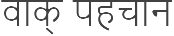
\includegraphics[width=1in]{../figs/vaakpahachaan.png}}}$$>$};
    \node[boxed] (n1) at (-0.75,1) {Pronunciation FST,\\$\rho(\phi|w)$} 
    edge[pre2](n0);
    \node[boxed] (n2) at (2.5,1) {Misperception FST,\\$\rho(\psi|\phi)$}
    edge[pre2] (n1);
    \node[boxed] (n3) at (5.75,1) {Phoneme-to-grapheme FST, $\rho(\lambda|\psi)$}
    edge[pre2] (n2);
    \node[open] (n4) at (9,1) {$\lambda$: Annotation-language orthography\\$<$vak paychan$>$} 
    edge[pre2](n3);
    \node[open] (n5) at (1,-1.5) {$\phi=$Utterance phones\\\ipa{[va:k p@H@tSa:n]}};
    \node[open] (n6) at (4,-1.5) {$\psi=$Perceived phones\\\ipa{[vAk p\textsuperscript{h}eItSAn]}}; 
  \end{tikzpicture}\\
\end{center}
\setlength{\abovecaptionskip}{0pt}
\caption{Mismatched Crowdsourcing: crowd workers on the web are asked
  to transcribe speech in a language they do not know.  Annotation
  mistakes are modeled by a finite state transducer (FST) model of
  utterance-language pronunciation variability (reduction and
  coarticulation), composed with an FST model of non-native speech
  misperception (mapping utterance-language phones to
  annotation-language phones), composed with an inverted
  grapheme-to-phoneme (G2P) transducer.}
\label{fig:h2e_eg2}
\end{figure}

In~\cite{JHJ15a}, a methodology was proposed that bypasses the need
for native language transcription: mismatched crowdsourcing sends target
language speech to crowd-worker transcribers who have no
knowledge of the target language, then uses explicit mathematical
models of second language phonetic perception to recover an equivalent
phonetic transcript (Fig.~\ref{fig:h2e_eg2}).  Majority voting is
re-cast, in this paradigm, as a form of error-correcting code
(redundancy coding), which effectively increases the capacity of the
noisy channel; interpretation as a noisy channel permits us to explore
more effective and efficient forms of error-correcting codes.
Assume that cross-language phone misperception is a finite-memory
process, and can therefore be modeled by a finite state transducer
(FST).  The complete sequence of representations from utterance
language to annotation language can therefore be modeled as a noisy
channel represented by the composition of up to three consecutive FSTs
(Fig.~\ref{fig:h2e_eg2}): a pronunciation model, a misperception
model, and an inverted grapheme-to-phoneme (G2P) transducer.
%MH 3/22/2016: following material is redundant with the figure caption
%The
%pronunciation model is an FST representing processes that distort the
%canonical phoneme string during speech production, including processes
%of reduction and coarticulation.  The misperception model represents
%the mapping of the uttered phone string (in symbols matching the
%phone set of the spoken language) to the perceived phone string (in
%symbols matching the phone set of the annotation language).  Finally,
%the transcriber maps heard phones to nonsense words in the annotation
%language; the mapping from phones to orthography is an inverted G2P.

